\section{سوال چهارم}

همانطور که در تمرین قبل بیان شد، تلفن‌های همراه برنامه‌های متفاوتی را اجرا می‌کنند. برای این تمرین همان مفروضات برقرار است. که ۰٫۵ وات در هر هسته و Core Quad ایمیل ۳ برابر سریع‌تر است.


\begin{enumerate}
	\item تصور کنید که ۸۰ درصد کد قابل موازی‌سازی است. فرکانس و ولتاژ روی یک هسته چقدر باید افزایش یابد تا با همان سرعت کد به صورت Parallelized Way Four اجرا شود؟
	\begin{qsolve}
طبق قانون Amdahl داریم:
	\begin{equation}
		\frac{1}{\frac{0.5}{4+0.2}} = \frac{1}{0.2+0.2} = \frac{1}{0.4} = \mathcolorbox{yellow}{2.5}
	\end{equation}
	\end{qsolve}







	\item کاهش انرژی دینامیکی ناشی از استفاده از مقیاس فرکانس و ولتاژ در قسمت قبل چقدر است؟
	\begin{qsolve}
برای ۴ هسسته که هر کدام با نسبت $\frac{1}{2.5}$ فرکانس و ولتاژ هستند داریم:
	\begin{equation}
		Energy: \frac{Energy_{quad}}{Energy_{single}} = 4 \times \frac{(V \times \frac{1}{2.5})^2}{V^2}=\mathcolorbox{yellow}{0.64}
	\end{equation}
	
	\begin{equation}
		Power: \frac{Power_{new}}{Power_{old}} = 0.64 \times \frac{f \times \frac{1}{2.5}}{f}=\mathcolorbox{yellow}{0.256}
	\end{equation}
	\end{qsolve}







	\item چه مقدار انرژی با رویکرد سیلیکون تاریک مصرف می‌شود؟ در این رویکرد، تمام واحد‌های سخت افزاری دارای قابلیت قطع کردن منبع تغذیه هستند و به آنها اجازه می‌دهد تا به طور کامل خاموش شوند. ASIC ها خاص منظوره به این دلیل ارائه شده اند که محاسبات مشابهی را تنها با ۲۰ درصد توان پردازشگر خاص منظوره انجام دهند. تصور کنید که هر هسته دارای قابلیت ثطع منبع توان است. همچنین یک بازی ویدئویی به دو ASIC و دو هسته نیاز دارد. با این مفروضات، چه مقدار انرژی دینامیکی در مقایسه با حالت موازی شده پایه‌ای روی چهار هسته نیاز است؟
	\begin{center}
		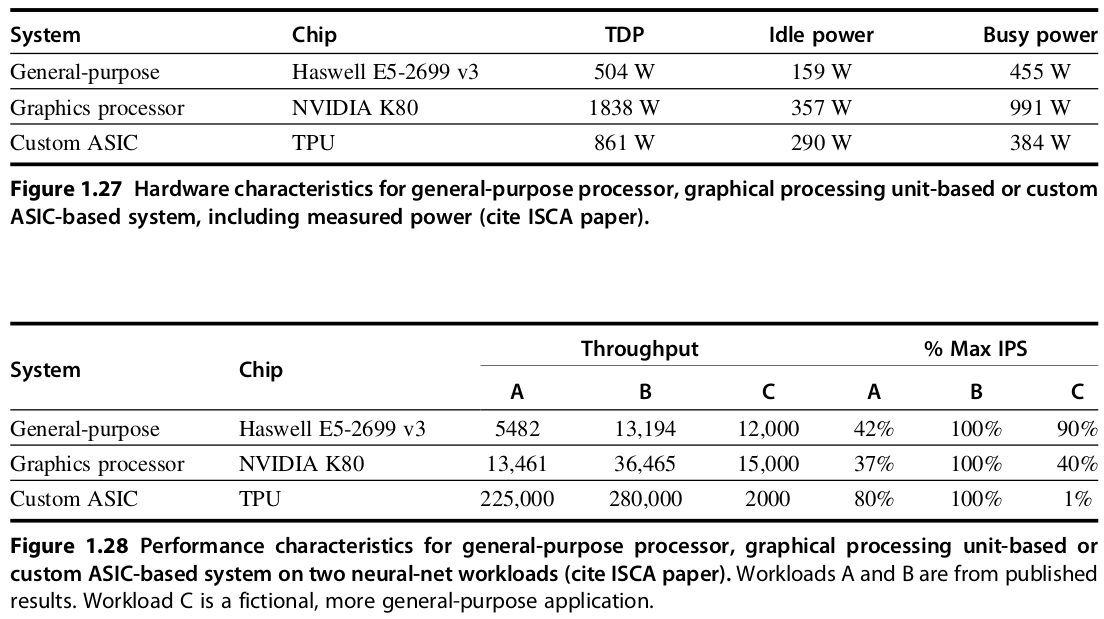
\includegraphics[scale=0.4]{pics/img1.png}
	\end{center}
	

	\begin{qsolve}
برای ۲ هسته + ASIC 2 در برابر ۴ هسته داریم:
	\begin{equation}
		\frac{2 + (0.2 \times 2)}{4} = \frac{2.4}{4} = \mathcolorbox{yellow}{0.6}
	\end{equation}
	\end{qsolve}







\end{enumerate}